\chapter{Problem statement}
\label{ch:chap1}

Tracking underwater objects, which refers to the continuous and accurate estimation of a target's position within a video sequence captured underwater, is a critical task with significant implications for marine applications. These applications span across environmental monitoring, resource development, and ecological protection \cite{qiu2024boundary}, where precise tracking can aid in assessing marine ecosystems, monitoring aquatic life, and ensuring the sustainability of ocean resources. However, the unique characteristics of the underwater environment introduce substantial challenges that complicate the task of object tracking in this setting.

One of the foremost challenges is the issue of \textbf{water turbidity and blurring effects}. Underwater optical images are frequently affected by turbidity, which results in significant blurring and fog. This occurs due to the absorption and scattering of light by seawater and various suspended particles, including minerals, salt, sand, and plankton \cite{zhou2024real, elmezain2025advancing, bhadouriaunderwater}. The turbid nature of water severely limits visibility, introducing haze that further complicates the clarity of captured images. Additionally, turbulence in the water flow can cause motion blur, which further disrupts the tracking process and reduces the precision of object localization \cite{bhadouriaunderwater}.

% example water turbidity and blurring effects
\begin{figure}[ht]
    \centering
    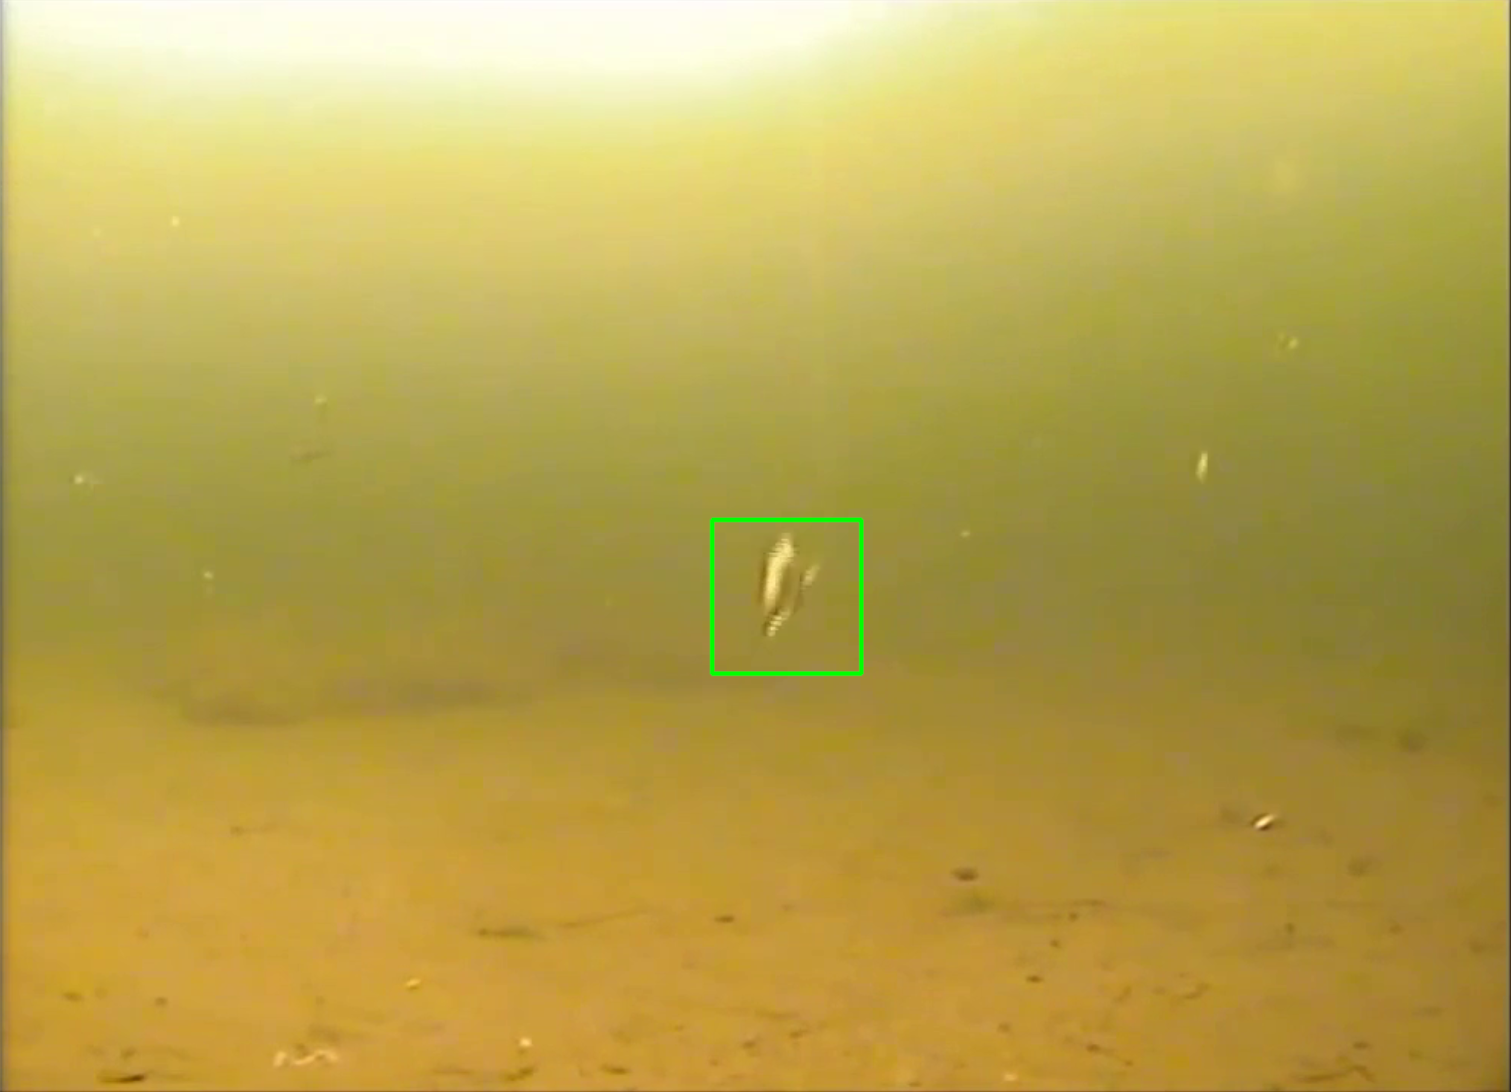
\includegraphics[width=0.8\textwidth]{images/water turbidity and blurring effects.png}
    \caption{Example of water turbidity and blurring effects. Source: UOT100 dataset \cite{kezebou2019underwater}.}
    \label{fig:turbidity}
\end{figure}


Another obstacle faced in underwater tracking is \textbf{color attenuation and light scattering}. As light travels through water, different wavelengths are absorbed at varying rates, with red light being absorbed more rapidly than other wavelengths \cite{elmezain2025advancing}. This phenomenon leads to the attenuation of color, which distorts the natural hues of objects and affects the overall image quality. The scattering of light by suspended particles further diminishes light intensity and alters its direction, resulting in color distortion that can make it even more difficult to distinguish between different objects. This attenuation of color and reduction in light intensity contribute to the overall decolorization of underwater scenes, posing a significant challenge for accurate object tracking \cite{elmezain2025advancing, bhadouriaunderwater, rout2019walsh}.
% Bluelike
\begin{figure}[ht]
    \centering
    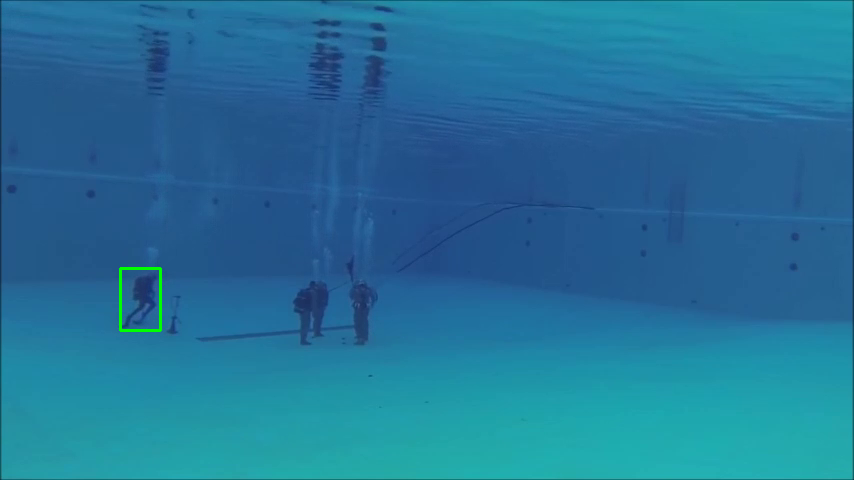
\includegraphics[width=0.9\textwidth]{images/color attenuation and light scattering.png}
    \caption{Example of color attenuation and light scattering. Source: UOT100 dataset \cite{kezebou2019underwater}.}
    \label{fig:color attenuation}
\end{figure}

In addition to these optical challenges, \textbf{low-contrast targets and occlusion} are persistent problems in underwater environments. Low visibility, low contrast, and low light intensity are common characteristics of underwater images, making it particularly difficult to discern objects and extract meaningful features for tracking \cite{zhou2024real, bhadouriaunderwater}. Moreover, many marine species exhibit camouflage, blending seamlessly with their surroundings, which complicates the process of segmentation and accurate identification \cite{elmezain2025advancing}. Furthermore, occlusion, where one object partially or fully obscures another, presents a substantial problem. This can significantly hinder the ability to maintain a consistent track of the target, especially in dynamic environments where objects frequently move in and out of view \cite{zhou2024real, elmezain2025advancing, mathias2022occlusion}.

% example low-contrast targets and occlusion
\begin{figure}[ht]
    \centering
    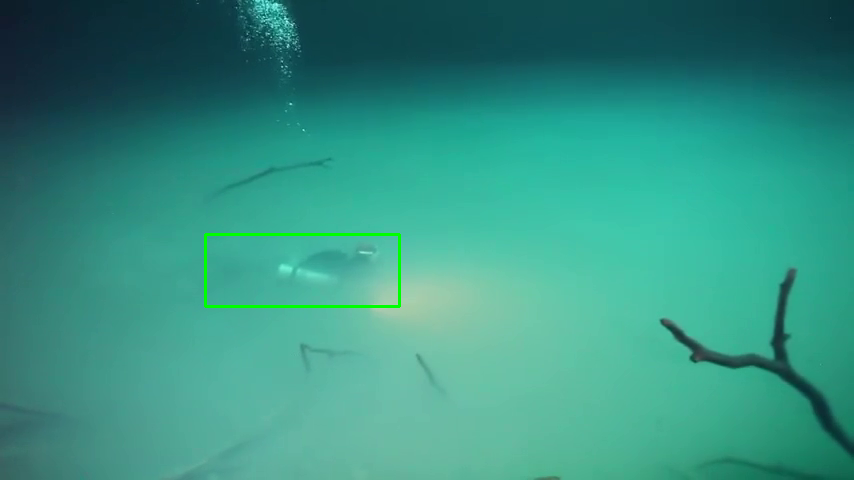
\includegraphics[width=0.8\textwidth]{images/CenoteAngelita.png}
    \caption{Example of low-contrast targets and occlusion. Source: UOT100 dataset \cite{kezebou2019underwater}.}
    \label{fig:low-contrast}
\end{figure}

The underwater environment is also characterized by \textbf{dynamic backgrounds with similar-looking objects}, adding another layer of complexity. Marine organisms exhibit a wide range of sizes and shapes, often appearing in dense clusters or schools, such as schools of fish. The presence of these similar-looking objects in the background can lead to confusion, as tracking algorithms may mistakenly identify these objects as the target, causing errors and drift in the tracking process \cite{zhang2024webuot}. The complexity and dynamic nature of the underwater scene further exacerbate the challenges faced by tracking algorithms.
% example dynamic backgrounds with similar-looking objects
\begin{figure}[ht]
    \centering
    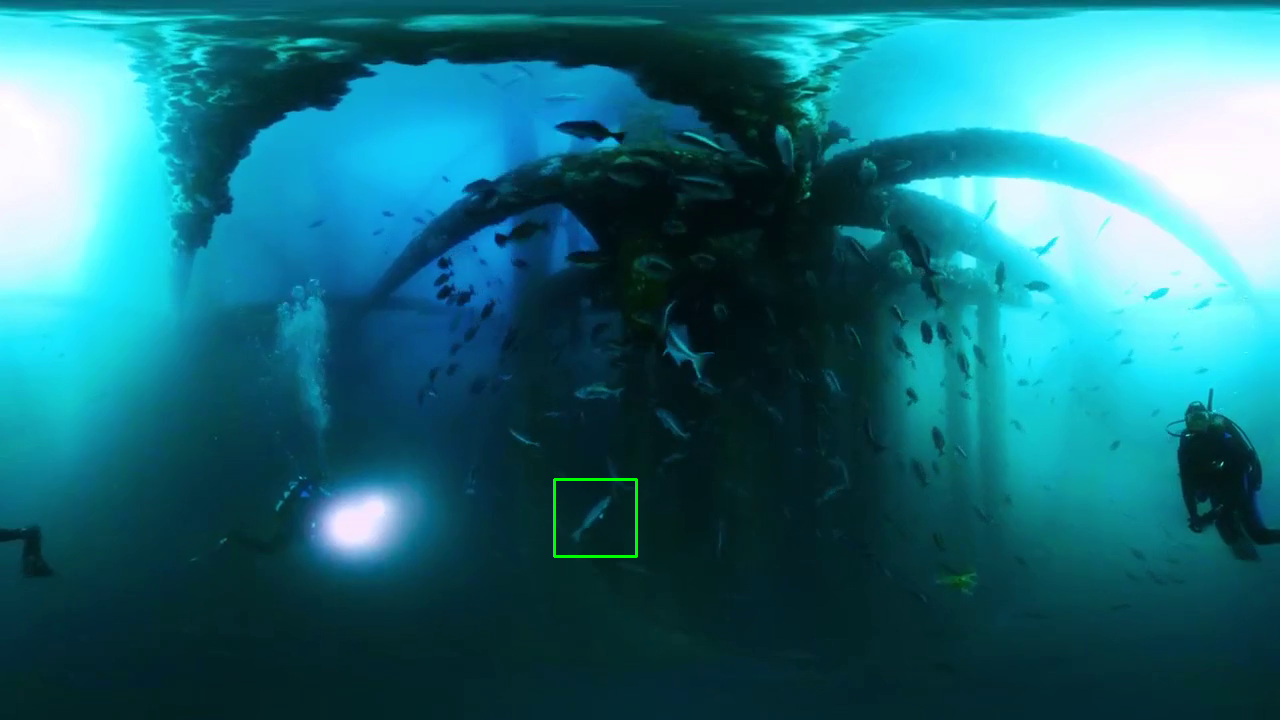
\includegraphics[width=0.8\textwidth]{images/Diving360Degree2.png}
    \caption{Example of dynamic backgrounds with similar-looking objects. Source: UOT100 dataset \cite{kezebou2019underwater}.}
    \label{fig:dynamic backgrounds}
\end{figure}

Traditional object tracking methods, primarily designed and optimized for open-air environments, struggle to perform effectively in underwater settings \cite{elmezain2025advancing}. These conventional methods are not robust enough to handle the significant domain shifts introduced by the optical properties of water, such as color distortion, image blur, and light scattering \cite{elmezain2025advancing}. Moreover, mainstream tracking models can be computationally expensive, often requiring high computational power that may not be available on resource-constrained underwater edge devices \cite{qiu2024boundary}. The inherent challenges of target feature distortion and contrast attenuation in underwater scenes can further undermine the ability of general tracking algorithms to differentiate between the target and its background, reducing their reliability. Therefore, specialized tracking models that take into account the unique characteristics of the underwater environment, along with underwater-specific datasets, are essential for improving the accuracy and reliability of object tracking in such challenging conditions \cite{elmezain2025advancing}.

\endinput